

\documentclass[twoside,twocolumn]{article}

\usepackage{blindtext} % Package to generate dummy text throughout this template 
\usepackage{graphicx}
\usepackage[sc]{mathpazo} % Use the Palatino font
\usepackage[T1]{fontenc} % Use 8-bit encoding that has 256 glyphs
\linespread{1.05} % Line spacing - Palatino needs more space between lines
\usepackage{microtype} % Slightly tweak font spacing for aesthetics

\usepackage[english]{babel} % Language hyphenation and typographical rules

\usepackage[hmarginratio=1:1,top=32mm,columnsep=20pt]{geometry} % Document margins
\usepackage[hang, small,labelfont=bf,up,textfont=it,up]{caption} % Custom captions under/above floats in tables or figures
\usepackage{booktabs} % Horizontal rules in tables

\usepackage{lettrine} % The lettrine is the first enlarged letter at the beginning of the text

\usepackage{enumitem} % Customized lists
\setlist[itemize]{noitemsep} % Make itemize lists more compact

\usepackage{abstract} % Allows abstract customization
\renewcommand{\abstractnamefont}{\normalfont\bfseries} % Set the "Abstract" text to bold
\renewcommand{\abstracttextfont}{\normalfont\small\itshape} % Set the abstract itself to small italic text

\usepackage{titlesec} % Allows customization of titles
\renewcommand\thesection{\Roman{section}} % Roman numerals for the sections
\renewcommand\thesubsection{\roman{subsection}} % roman numerals for subsections
\titleformat{\section}[block]{\large\scshape\centering}{\thesection.}{1em}{} % Change the look of the section titles
\titleformat{\subsection}[block]{\large}{\thesubsection.}{1em}{} % Change the look of the section titles

\usepackage{fancyhdr} % Headers and footers
\pagestyle{fancy} % All pages have headers and footers
\fancyhead{} % Blank out the default header
\fancyfoot{} % Blank out the default footer
\fancyhead[C]{Titulo $\bullet$ Junio 2019 $\bullet$ } % Custom header text
\fancyfoot[RO,LE]{\thepage} % Custom footer text

\usepackage{titling} % Customizing the title section

\usepackage{hyperref} % For hyperlinks in the PDF

%----------------------------------------------------------------------------------------
%	TITLE SECTION
%----------------------------------------------------------------------------------------

\setlength{\droptitle}{-4\baselineskip} % Move the title up

\pretitle{\begin{center}\Huge\bfseries} % Article title formatting
\posttitle{\end{center}} % Article title closing formatting
\title{Auditoria de Bases de datos} % Article title
\author{Richard cruz Escalante  Codigo : 2013047247}
\date{\today} % Leave empty to omit a date
\renewcommand{\maketitlehookd}{%

}

%----------------------------------------------------------------------------------------

\begin{document}

% Print the title
\maketitle

%----------------------------------------------------------------------------------------
%	ARTICLE CONTENTS
%----------------------------------------------------------------------------------------

\section{Introduccion}
\lettrine[nindent=0em,lines=3]{E}s el proceso que permite medir, asegurar, demostrar, monitorear y registrar los accesos a la información almacenada en las bases de datos incluyendo la capacidad de determinar:
\\
– Quién accede a los datos.
\\
– Cuándo se accedió a los datos.
\\
– Desde qué tipo de dispositivo/aplicación.
\\
– Desde que ubicación en la Red.
\\
– Cuál fue la sentencia SQL ejecutada.
\\
– Cuál fue el efecto del acceso a la base de datos.

%------------------------------------------------

\section{Objetivos}

\begin{itemize}

\item Mitigar los riesgos asociados con el manejo inadecuado de los datos.
\item Apoyar el cumplimiento regulatorio.
\item Satisfacer los requerimientos de los auditores.
\item Evitar acciones criminales.
\item Evitar multas por incumplimiento.
\end{itemize}




%------------------------------------------------

\section{Marco teorico}

\subsection{Azure Data studio}
Azure Data Studio es una herramienta de base de datos multiplataforma para profesionales de datos que utilizan la familia de plataformas de datos en la nube y locales de Microsoft en Windows, MacOS y Linux.

Anteriormente publicado bajo el nombre de vista previa de SQL Operations Studio, Azure Data Studio ofrece una experiencia de edición moderna con IntelliSense, fragmentos de código, integración de control de fuente y un terminal integrado. Está diseñado teniendo en cuenta al usuario de la plataforma de datos, con un registro integrado de conjuntos de resultados de consulta y paneles personalizables.

\begin{center}
	
\includegraphics[width=5cm]{./Imagenes/azure} 
\end{center}


\section{Desarrollo}

\subsection{Paso 1}
Creando auditoria con las siguientes propiedades
\begin{center}
	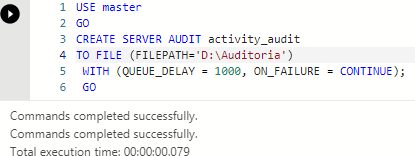
\includegraphics[width=5cm]{./Imagenes/1} 
\end{center}
\subsection{Paso 2}
Activar auditoria
\begin{center}
	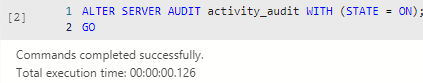
\includegraphics[width=5cm]{./Imagenes/2} 
\end{center}
\subsection{Paso 3}
Crear una especificacion de auditoria
\begin{center}
	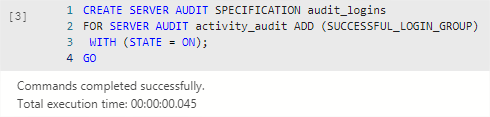
\includegraphics[width=5cm]{./Imagenes/3} 
\end{center}
\subsection{Paso 4}
Activar la especificacion
\begin{center}
	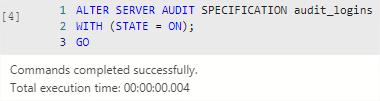
\includegraphics[width=5cm]{./Imagenes/4} 
\end{center}
\subsection{Paso 5}
Crear yba especificacion de auditoria de base de datos salesapp1
\begin{center}
	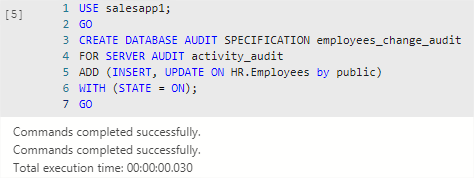
\includegraphics[width=5cm]{./Imagenes/5} 
\end{center}
\subsection{Paso 6}
Activar la especificacion de auditoria de la DB
\begin{center}
	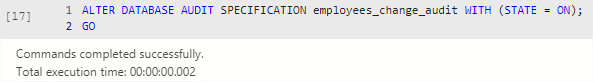
\includegraphics[width=5cm]{./Imagenes/6} 
\end{center}
\subsection{Paso 7}
Ejecutar el codigo, escribir una consulta de sistema sys fn get audit file para devolver todos los datos de auditoria desde los archivos en D:Auditoria, filtrar los datos para que solo la actividad relacionada a la sesion actual sea visualizada.
\begin{center}
	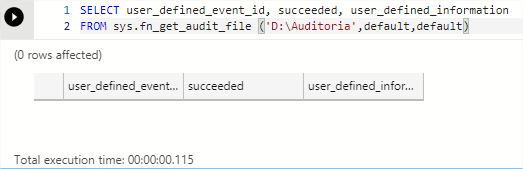
\includegraphics[width=5cm]{./Imagenes/7} 
\end{center}
\subsection{Paso 8}
Deshabilitar la auditaria del servidor activity audit
\begin{center}
	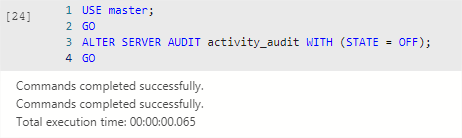
\includegraphics[width=5cm]{./Imagenes/8} 
\end{center}
%	REFERENCE LIST
%----------------------------------------------------------------------------------------


%----------------------------------------------------------------------------------------

\end{document}
